\section{Analysis}
\subsection{Problem Defenition}
The goal of this project is to design the hardware specification for a custom CPU, and develop the suite of tools required for a programmer to write programs for this processor. This will involve writing an Emulator (\ref{sec:Emulator}), Assembler (\ref{sec:Assembler}), and Compiler (\ref{sec:Compiler}). The project will detail the abstract design of the computer’s Instruction Set Architecture (ISA) (\ref{sec:ISA}) and its implementation in hardware, considering the internal registers, system clock, main memory, and fetch execute cycle.

The project will compose three primary parts, an emulator capable of loading machine code 'catridges' and simulating the hardware behaviour required to execute them with correct clock timing and behaviour. An assembler to translate programs written in an assembly language into binary machine code. And finally a compiler - to translate a higher level programming langauge into machine code. This will require compiler optimisations in the produced object code; complex data structures such as arrays, objects and strings; conditional and iterative expressions; and finally functions and procedures. All together, the processor and suite surrounding it should be capeable of writing and compiling complex programs such as pong or tetris, and emulating them with hardware correct timings - dealing with I/O peripherals such as a keyboard or speaker.

\subsection{Background to the Problem Area}
I have a keen curiosity around the lower level elements of software development, and this project will help me understand how the everyday langauges I use to program are implemented from the processor level upwards. It will look in detail at the fundemental architecture of modern computing systems and how they are developed, looking in particular at the process of designing a processor and corresponding machine code specification with an assembler and compiler to allow a programmer to write programs to run on this computer. Below I will perform some initial research into what these 4 components of the system would entail:

\subsubsection{Instruction Set Architecture}
\label{sec:ISA}
The ISA acts as an interface between the hardware and software of a computing system, it contains crucial information regarding the capabilities of a processor, including: a functional defenition of storage locations (e.g. registers and memories) as well as a description of all instructions and operations supported. An important consideration will be whether to design an 8 or 16 bit system, 16-bits would allow for more complex instructions and operations to be executed in a single cycle since more bits can be processed by the CPU simultaneously, however an 8 bit system is more efficient and simpler to design and emulate since considerations like whether to use little or big endian encodings can be ignored (whether to store the most significant byte of a 16-bit integer before or after the least significant).

An ISA can be classified according to its architectural comlpexity into a Complex Instruction Set Computer (CISC), or a Reduced Instruction Set Computer (RISC). A CISC processor implements a wide variety of specialized instructions in hardware (e.g. floating point arithmetic or transferring multiple registers to or from the stack), minimising the number of instructions per program at the cost of a more complex design, higher power consumption and slower execution as each instruction requires more processor cycles to complete. \textcite{gfg-risc-vs-cisc} Thus optimisations in performance occur on the hardware level. This is historically the most common branch of processor and often results in large instruction sets, for example the Intel x86's 1503 defined instructions \textcite{ryg-blog}. A RISC processor however aims to simplify hardware using an instruction set consisting of a few basic instructions to load, evaluate and store data. This has the side effect of increased memory usage, as memory is required to store the additional instructions needed to perform the complex tasks not implemented in hardware.

\subsubsection{Emulator}
\label{sec:Emulator}
An emulator is a software program that allows the host computer to replicate the hardware of the target machine. It reads machine code instructions assembled for the target computer from memory and interprets them, mimicing the internal state of the target machine in the process, \textcite{CHIP-8-blog}. Emulators consist of three modules, a CPU emulator, memory subsystem, and I/O device emulators, \textcite{retroreversing}. The simplest form of CPU emulator is an interpreter - wherein the emulator steps sequentially through each machine code instruction, and carries out the fetch-decode-execute cycle, modifying the internal state of the simulated processor in the same manner the instruction would affect the physical hardware. The Memory Subsystem is a one dimensional array of bytes that can be addressed in the same manner as RAM, regions of memory are allocated to peripherals and subsystems as with a real processor, e.g. Video Random Access Memory (VRAM), the stack, and the heap. Finally, I/O device emulators translate the input from your keyboard into device specific command signals that the processor can interface with.

\subsubsection{Assembler}
\label{sec:Assembler}
An assembler is a program that translates assembly language (a low level programming language that uses mneumonics to directly represent machine code instructions) into object code that can be executed by the processor. There are 2 types of assembler design, single-pass and multi-pass \textcite{TOPPR-assembler}. A single-pass assembler scans the source code only once to translate it into machine code, and outputs the result directly. This is the simpler type of assembler, and has faster translation speeds. However, it requires all symbols used within the program (variables, labels, etc...) to be declared before they are used - else the program will crash. 

A multi-pass assembler however scans the source code multiple times, on the first pass it defines a symbol and opcode table (mapping instructions and variables to their memory address which can be queried by the assembler when calculating offsets) \textcite{TOPPR-assembler}, processes pseudo instructions (compound macro instructions that are substituted during assembly with a list of fundemental instructions performing that complex task), and maintaining a location counter to store the memory address of each instruction as it would be compiled.

There are also certain higher level abstractions a high-level assembler can translate such as \texttt{IF/THEN/ELSE/WHILE} statements and certain higher level data types – however this results in a complex assembler and lengthy compilation times - as well as a blurred line between the role of high level and low level languages. 

\subsubsection{Compiler}
\label{sec:Compiler}
A compiler is a program that translates high level program source code into a set of machine language instructions. Some compilers translate source code into an intermediate assembly language before using an assembler to produce the machine code instructions, whereas others compile into machine code directly. The typical pipeline to any compiler is depicted in fig. \ref{fig:compiler-pipeline} \textcite{Ball-WritingACompilerInGo}.

\bigskip

\begin{figure}%
    \centering
    \subfloat[\centering Compiler Pipeline]{{
        \shadowbox{
            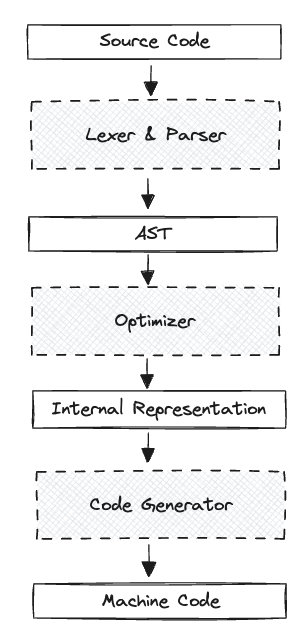
\includegraphics[height=6cm]{Screenshot 2024-04-21 at 14.52.32.png}
        }
        \label{fig:compiler-pipeline}%
        }}%
    \qquad
    \subfloat[\centering Abstract Syntax Tree]{{
        \shadowbox{
            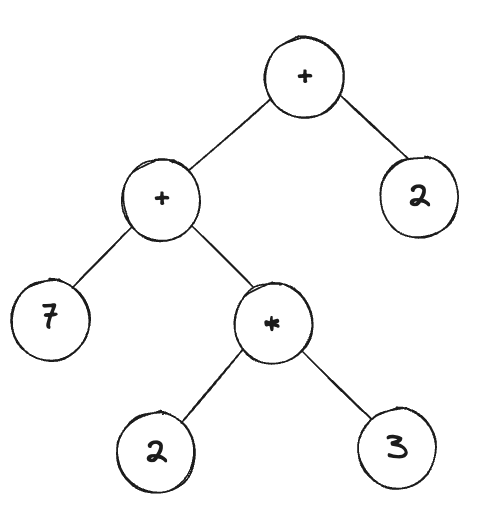
\includegraphics[height=6cm]{Screenshot 2024-04-21 at 15.01.11.png}
        }
        \label{fig:ast}%
    }}%
\end{figure}

\bigskip


A compiler is composed of three parts working in unison, Lexical analysis, Parsing, and Code Generation. The ASCII source code is tokenised by the lexer - meaning it is broken down into a list of its fundemental elements (e.g. strings, integers, keywords), and fed into the Parser where it is transformed into an Abstract Syntax Tree (AST) representing the structure of the program. 

The AST is a means of breaking down the program, its statements, and order of operations into a tree representation that is easier to be processed and traversed by an algorithm. The AST representing expression ($\frac{7+2\times3}{2}$) is depicted in fig. \ref{fig:ast}. 

The optimizer may convert the AST into an Internal Representation (IR) (be that binary, textual, or another syntax tree) which is another means of representing the data in a form that lends itself better to optimisations and translation into the target language than the AST. From this new IR, optimisations may include eliminating dead code, precalculating simple arithmetic, and numerous other optimisations \textcite{Ball-WritingACompilerInGo}. Finally, the code generator generates the optimised code in the target language (compilation) and is stores it as a file on the user's computer.



\bigskip

\bigskip

\subsubsubsection{Lexer}
The first component of a compiler, the lexer steps through the ASCII source code character by character and builds up tokens representing the basic elements of a program such as a String, Integer, Identifier, Keyword. For example the program: \texttt{print("Result: ", (answer+1)/2)} would be tokenised as:

\begin{lstlisting}
IDENTIFIER("print"), LPAREN, String("Result: "), COMMA, LPAREN, IDENTIFIER("answer"), ADD, INTEGER(1), RPAREN, DIV, INTEGER(2), RPAREN
\end{lstlisting}

This process of tokenising the program string into a series of objects makes it easier to parse into an AST and for the parser to step through by element rather than character.

\subsubsubsection{Parser}
The process of converting the list of tokens representing the program generated by the Lexer into a tree representation (AST) that reflects the order of operations and sequence of statements is called Parsing. And is carried out by a Parser. There are two classifications of parsing algorithms, a top down parser and a bottom up parser.

A top-down parser builds its syntax tree from the root node, or highest level expressions (arithmetic operations, selective or iterative statements) and works its way down into the atomic (or leaf) nodes of the graph (individual numbers or variables). A bottom-up parser however begins with an atom such as an integer and continues to scan the source code - building up a picture of the syntax tree. For example, should the parser encounter an integer, it would continue scanning and were the next character to be an operation - the parser would know the statement must be an infix arithmetic operation, thus can transpose the graph into one representing a statement in that form (ie a root node with two children nodes for the left and right hand side of the operation). Repeating this process throughout the file builds up a syntax tree representing the program as a whole.

\subsubsubsection{Optimization \& Code Generation}
Code generation is the process of converting the AST generated from the Parser into an intermediate language which itself can be compiled down to an executable or interpreted by a virtual machine. For my NEA, the compiler will first compile down into assembly language - which will then be assembled into the executable machine code - simplifying compilation through the available higher level functionality such as labels and offsets. Each higher level statement typically templates onto a standard sequence of machine code instructions, for example a program to add 2 numbers:
\begin{lstlisting}
let a = 9;
let b = 5;
let c = a + b;
\end{lstlisting}
\begin{lstlisting}
ldi R0, 9
ldi R1, 5
add R2, R0, R1
\end{lstlisting}
Compilations such as these involve the mapping of a potentially infinite number of variables onto a discrete number of regiseters, and this can be performed using such algorithms as the Linear Scan or Chatins' algorithm \textcite{GFG-linearscan} that take into account variable lifetimes and interactions. Offsets required for branch instructions that may be used in iterative or selective statements can be calculated by counting the number of instructions compiled up to the point of a particular statement (e.g. the number of machine code instructions up the the condition of a while loop) and this can be used as either an absolute or relative offset depending on the capabilities of the assembler.

\subsection{Existing Systems}
\subsubsection{University of Washington MIPS Computer}
\label{sec:UoW}
The following system is a 16 bit MISC (Minimal Instruction Set Computer) processor designed by the University of Washington for a series of lectures as part of their computer science course \textcite{MIPS-uw}, and I will discuss its ISA and machine code encoding - to aid my design of an appropriate and efficient computer architecture. A MISC processsor is a subclass of the RISC processor and involves minimising the number of instructions implemented in hardware, resulting in far simpler hardware designs - where a RISC processor may have 30-70 instructions, a MISC processor may have merely 10-20 consisting of arithmetic, branching, loading and storing instructions. \textcite{MISC-dakeng}. 

A MIPS (Microprocessor without Interlocked Pipelined Stages) processor such as this does not overlap the execution of several instructions (pipelining), thus neglecting the potential performance gains in favor of a simpler architecture. This processor is a single-cycle implementation meaning all instructions take exactly one cycle to complete, this is achieved using a Harvard architecture in place of Von Neuman wherein instructions are stored in a seperate Read Only Memory (ROM) to data, thus both can be fetched within the same processor cycle. 

The processor supports the following instructions:
\begin{enumerate}
    \item Arithmetic \texttt{add, sub, and, or, slt (set if less than)}
    \item Data Transfer \texttt{lw (load word), sw (store word)}
    \item Control \texttt{beq (branch if equal to)}
\end{enumerate} 
Register-to-Register arithmetic instructions use the R-type encoding for their machine code representation, where \texttt{op} is the opcode of the instruction, \texttt{func} the control bits for that particular arithmetic operation, and \texttt{rs, rt}, and \texttt{rd} being the source and destination registers respectively. This computer operates on an ALU with a 3 bit control signal supporting 5 operations that directly correspond to the \texttt{func} portion of an R type instructions binary encoding. 

\bigskip

\shadowbox{
    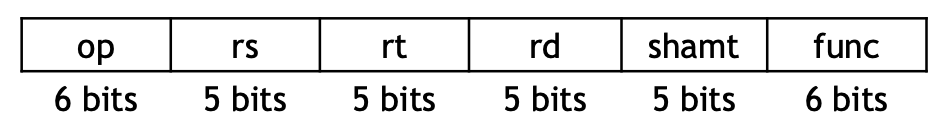
\includegraphics[width=11cm]{Screenshot 2024-04-14 at 22.19.47.png}
}

\bigskip

The I type encoding is the second means for which instructions can be represented, and includes the data transfer and control instructions \texttt{lw, sw}, and \texttt{beq} specified above. \texttt{address} is a signed 16 bit constant. \texttt{rt} is the destination for \texttt{lw} and source for \texttt{beq} and \texttt{sw}. \texttt{rs} is the base register for the \texttt{lw} and \texttt{sw} instructions (added to the signed constant \texttt{address} to get a data memory address) \textcite{MIPS-uw}. In this processor design, in a \texttt{beq} instruction, the \texttt{address} field specifies not a memory address, but a signed offset from which to jump from the current PC position when executing the branch instruction.

\bigskip

\shadowbox{
    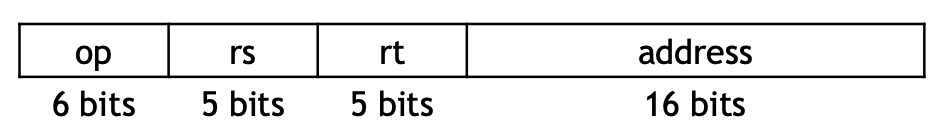
\includegraphics[width=11cm]{Screenshot 2024-04-14 at 22.33.16.png}
}

\bigskip

Below is the full datapath specification for the computer, with the Instruction Memory (ROM) on the left, connected to the PC in order to address instructions. Those instructions are in turn passed through the control unit and decoded, with the opcode specifying whether an I or R type instruction is being processed and accordingly what hardware should be used to interpret and execute the instruction. This dictates the calculation (if any) that is to be performed in the ALU - the output of which is stored in a seperate data memory.

Since instructions are stored in a seperate ROM, the address of the first instruction will always begin at 0 - this simplifies the calculation of offsets and labels in the assembler – since the assumption that the first instruction begins at address 0 will always hold true. However, branch instructions are handled unusually in this computer - instead of specifying the jump address, the signed offset from the current instruction is specified instead. This has the effect of making compilation easier as branch addresses do not need to be calculated by the assembler, however renders specific jumps to memory addresses (such as the location of an interrupt service routine or bootloader) difficult.

\bigskip

\shadowbox{
    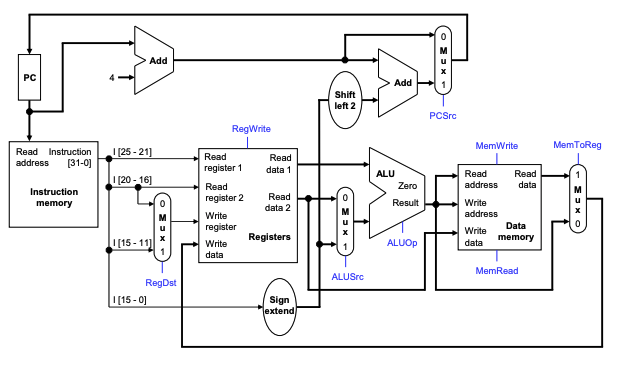
\includegraphics[width=11cm]{Screenshot 2024-04-14 at 19.42.11.png}
}

\subsubsubsection{Advantages \& Disadvantages}
The architecture described above has some notable advantages, firstly, its Harvard architecture allows the processor to operate each instruction in a single cycle – both improving performance and simplifying the design of the emulator as microinstruction cycles do not need to be simulated  to accurately simulate the hardware. Secondly, by dividing the computer architecture into 2 distinct I and R type instructions, you can reduce redundant information – and thus the bits required to store machine code instructions and programs.

However, this simple architecture results in many inconveniences when writing assembly code - due to the limited instruction set, simple tasks take comparatively more instructions meaning programs are longer and more tedious to write - as well utilising more memory due to the limited number of specialized instructions who's functionality must be implemented using handwritten subroutines such as binary shifts, stack operations, or interrupt handling. 

\bigskip

\subsubsubsection{Takeaways}
The takeaways of this system for my project include:
\begin{enumerate}
    \item I will consider using a Harvard architecture for my computer since all instructions can be single-cycle, thus simplifying design and emulation.
    \item The encoding of instructions into meaningful machine code that directly relates to the hardware of the computer - for instance R type opcodes representing the control bits of the ALU, this makes decoding instructions more efficient - especially when implemented in hardware.
    \item Secondly, the behaviour of hardware (registers, memories, flags) and the relationships between components during a single-cycle Harvard fetch-execute cycle that will have to be simulated when designing an emulator.
    \item I will also expand the instruction set further than the MISC specification used in this processor to include other common instructions, and keep the memory-register seperation wherin operations are performed on register values, with 2 instructions \texttt{lw, sw} used for reading and writing to memory.
    \item I will also change the branch instruction to operate on absolute addresses rather than signed offsets.
\end{enumerate}

\subsubsection{The Hack Computer}
The Hack computer is a theoretical 16 bit computer designed by Noam Nisan and Shimon Schocken and described in their book The Elements of Modern Computing Systems \textcite{EOCS}, I will analyse its method of encoding assembly instructions into machine code - as well as the syntax of its assembly language to inform my assembler design and machine code specification. The Hack computer contains 2 16-bit registers labelled A and D, the D (data) register is a general purpose register that always acts as 1 of the 2 inputs to the ALU. Wheras the A (address) register has 2 functions: a second signed integer value for ALU operations, and a target address in instruction memory or data memory addressing. The pseudo-M (memory) register is not implemented in hardware - rather refers to the word in RAM addressed by the A register and therefore can be used to directly interract and perform calculations with memory.
\begin{lstlisting}
A type: 0aaaaaaaaaaaaaaa
C type: 111accccccdddjjj
\end{lstlisting} 
Hack takes a unique aproach to ISA design through its address instructions (A-type) and computational instructions (C-type). The first bit of any machine code instruction determines its type. For an A instruction - the latter 15 bits store the data (or address) as which to set the A register (\texttt{a}). 

For a C-type instruction the the first 2 bits of the 15 bit operand remain unused and set to 1 by standard, this is followed by the 1 bit addressing mode (\texttt{a}) which determines whether A or M is used as the ALU's second input. Then, the computation specification (\texttt{c}) composes the next 5 bits, and dictate which operation the ALU will perform, directly mapping to the ALU's control bits \textcite{EOCS}. Following, the 3 bit destination specifier (\texttt{d}) in turn relate to the 3 'registers' A, D, and M. Should their corresponding bit be set the ALU output will be stored in the A, D or M registers (potentially multiple). The final 3 bits describe the jump condition - each Hack C type instruction is terminated by a branch (which can be left blank). They relate to the Less Than, Equal to, or Greater Than conditions respectively, and a combination can be used to form all conditionals.

\bigskip

\shadowbox{
    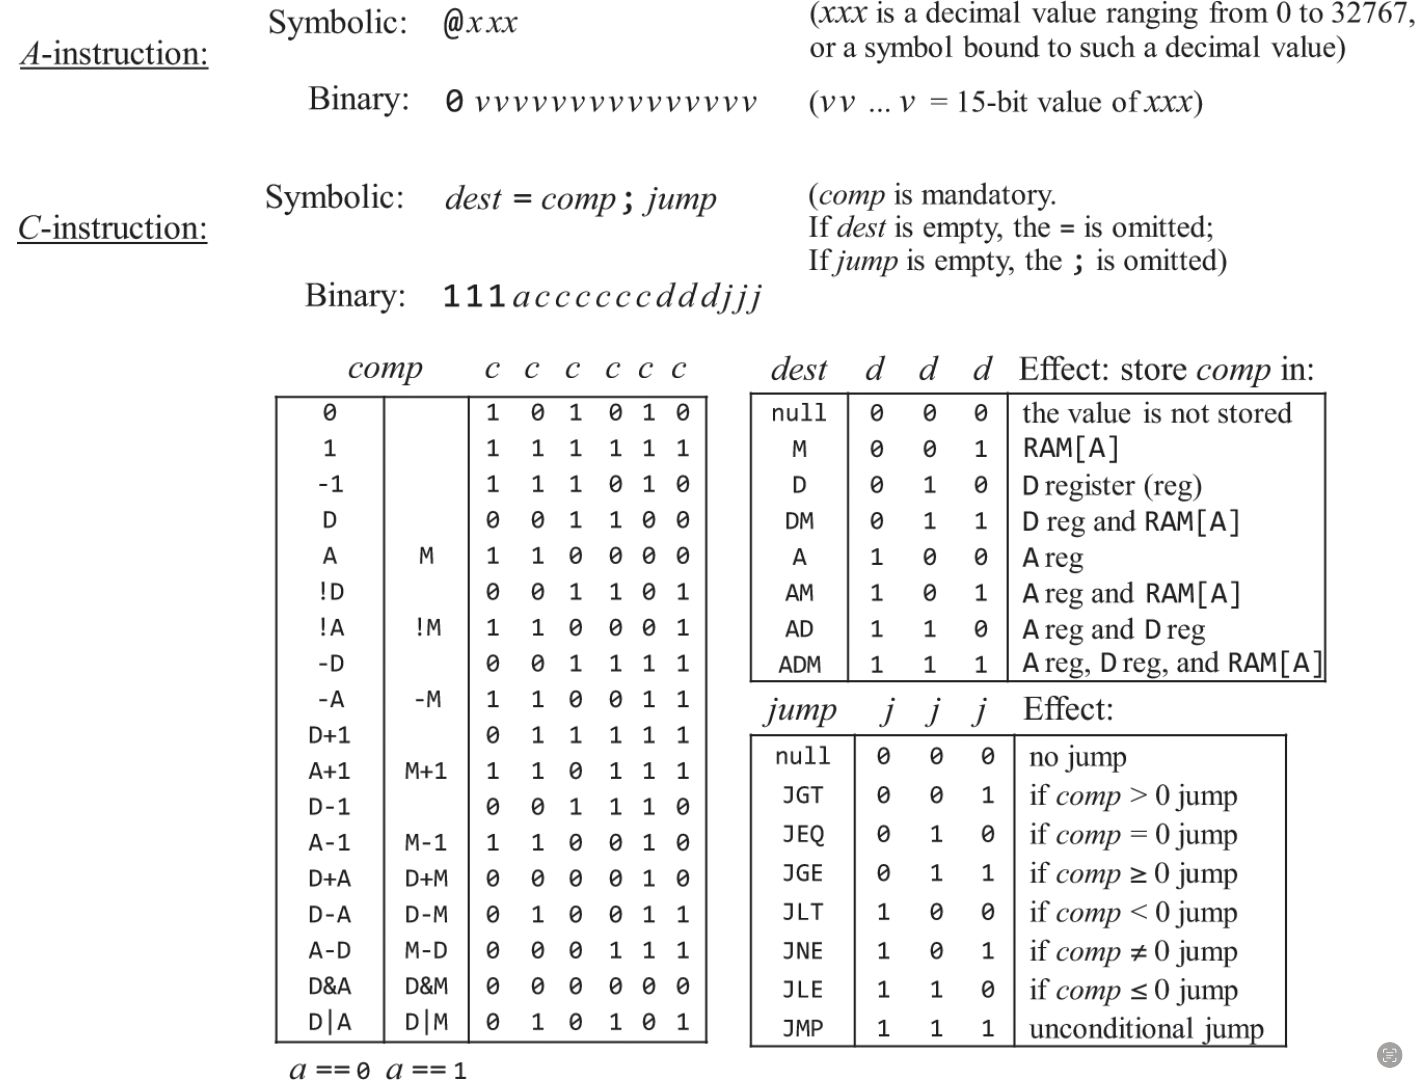
\includegraphics[width=11cm]{Screenshot 2024-04-21 at 17.17.34.png}
}

\bigskip

\subsubsubsection{Advantages \& Disadvantages}
This approach to ISA design being so fundementally related to the internal operations of the CPU comes with some advantages and disadvantages. Firstly, it is a very efficient design - allowing all essential operations to be carried out with a simple computer architecture. This simplicity makes it an ideal compilation target. However, Hack assembly can be unintuitive to write and understand - especially in relation to its Harvard architecture and thus simultaneous addressing of both instructions and data from ROM or RAM respsectively. An example Hack assembly program might look as follows:
\begin{lstlisting}
// i = 1
@i
M = 1

(LOOP)
    // if (i > 10) goto STOP
    @i 
    D = M

    @10
    D = D - A

    @STOP
    D; JGT

    // i += 1
    @i
    M = M + 1

    // goto LOOP
    @LOOP
    0;JMP
(STOP)
@END
0; JMP
\end{lstlisting}

Hack's approach to assembly is also worth considering, It uses parenthesis to specify labels (points in the code from which instructions can branch to without specifying a numeric offset). The '@' character is used to specify an A type instruction - however using an identifier as the operand is a high level assembler abstraction that at compile time replaces all occurrences of the identifier with a calculated memory address representing that variable. All C-type instructions are in the form \texttt{<destination(s)> = (<destination> <operation> <destination>)? (; <branch>)?} where the branch expression components of the instruction are optional. 

To compile this down into machine code (once labels have been replaced with offsets) - the A instruction is simply the 15 bit operand. The C instruction however is more involved. A lookup table is used to map the operations (\texttt{+, -, /, *, !, \&}) into 5 bit opcodes (with the first bit of the 6 bit computation specified determined by whether the A or M registers are included in the operands). Then the bit corresponding to each destination specified will be set, and finally the conditional branch bits will be set depending on the mneumonic used, e.g. \texttt{JGE} would be replaced by \texttt{011}. Together, the instruction \texttt{D = D - A; JNE} would be represented by the binary \texttt{111 010011 010 101}. 

\subsubsubsection{Takeaways}
From this case study, there are a number of takeaways:
\begin{enumerate}
    \item Breakdown instructions into types capable of representing a family of assembly insstructions - reducing the number of machine code instructions required to be implemented by the virtual machine.
    \item I will maintain a comparatively small instruction set, relying on macro instructions (compound instructions that are substituted at compile time for a list of fundemental ones carrying out that defined task) instead.
    \item Use a pseudo-register to represent the addressing behaviour of a Harvard architecture computer, simplifying operations involving memory access \& compilation behaviour.
    \item Represent branch conditionals through 3 bits reflecting \texttt{<, =, >} comparisons  
    \item Use one bit to represent each destination register allowing for a combination of destinations for a paricular instruction meaning seperate instructions need not be created for storing data in memory or registers.
\end{enumerate}

\subsubsection{Monkey}
Monkey is the programming language described in Thorsten Ball's book Writing a Compiler in Go \textcite{Ball-WritingACompilerInGo}, I will be analysing the syntax of the language to inform my high-level language design. Monkey has a C-like syntax, variables, integers and booleans, arithmetic expressions, first class functions (functions that can be passed to other functions as parameters), strings, and arrays. Its syntax looks as follows:
\begin{lstlisting}
let fibonacci = fn(x) {
    if (x == 0) {
        0;
    } else {
        if (x == 1) {
            1;
        } else {
            fibonacci(x - 1) + fibonacci(x - 2);
        };
    };
}

let main = fn() {
    let numbers = [1, 2, 10, 50, 9*18];
    let index = 0;

    while (index < length(numbers)) {
        print(fibonacci(numbers[index]));
        index = index + 1;
    }
}
\end{lstlisting}

\subsubsubsection{Advantages \& Disadvantages}
There are some advantages with this approach to language design, for instance its syntax lends itself to a simple and convenient to program parser, in particular, by representing functions as variables it allows you to pass functions as parameters (first order functions) without any additional logic validating return types or parameters. However, functionality as such is difficult to implement in machine code. Instead, passing the address of the first instruction of the function, rather than the function itself is a more practical solution for a compiled language. References and pointers are also not present in Monkey, these permit complex functionality such as arrays and strings, whilst maintaining a simple compiler since programmers can access variables by their location in memory rather than through an identifier (providing the ability to traverse an array through consecutive memory locations for example). However, this can lead to code that is difficult to understand and takes familiarity with the hardware \& implementation of the language to write. 

Monkey represents variables using Go's built-in data structures, thus doesn't have to compile them into binary - meaning specifying a data type is less important, and the language can afford to be dynamically typed - this means variable types are not checked when compiling expressions, and can result in runtime errors when attempting to add an integer to a string, or assign an integer to a float type variable. Using the \texttt{let} keyword to define a variable as above(unlike python) is vital for a compiled language - since additional functionality is required to allocate a memory address (or regiser) when declaring a variable depending on its lifetime.

\subsubsubsection{Implementation}
I will also look at the implementation of this language, in particular its Lexer and Parser as these are directly relevant to my NEA. Firstly, the Lexer. Monkey represents tokens as all deriving from an abstract class \texttt{Token} defined below.

\begin{lstlisting}
enum TokenType {
    LPAREN,
    RPAREN,

    STRING,
    IDENTIFIER,
    INTEGER,
    ...
}

type Token struct {
    enum TokenType
    Literal String
}
\end{lstlisting}

The code is scanned character by character and the fundemental elements of the program are stored in these token objects, for instance the string \texttt{"Hello, World!"} would be stored as \texttt{Token(TokenType::String, "Hello, World")}. A list of these token objects are returned by the lexer and used as input to the parser.

The Monkey interpreter's parser uses a top-down Pratt parser as opposed to the more common bottom-up parser.  Top-down parsers are simpler and more elegant to write due to their highly recursive nature - however this can make them troublesome to debug and maintain. They avoid much of the complex graph transpositions required for a bottom up parser.

\subsubsubsection{Takeaways}
The takeaways from this system include:
\begin{enumerate}
    \item Using established programming language norms for defining variables, iterative statements and functions will make the programming language easier to learn due to transferable experience.
    \item Designing a statically typed language would reduce program crashes and lead to a more robust compiler and programs.
    \item Including references and pointers allow for the implementation of features such as arrays and strings whilst maintaining a concise and simple compiler.
    \item I should consider defining variables with the 'let' keyword to tell the compiler it needs to insert additional logic calculating an appropriate memory address in which to store the variable, and store that address in a lookup table against its identifier.
    \item I should consider writing a top-down parser as opposed to a bottom up parser to ensure the code is cleaner, simpler and more elegant.
\end{enumerate}

\subsubsection{Jack}
Jack is the high level langauge defined in book The Elements of Modern Computing Systems \textcite{EOCS} with a syntax similar to Java. I will analyse its syntax and how it is compiled into machine code to inform my design of a compiled language. Jack is an Object-Oriented statically typed language similar to Java that is compiled down into the Hack machine code specification. An example Jack program may look as follows \textcite{EOCS}:
\begin{lstlisting}
class List {
    // declare the class attributes
    field int data;
    field List next;

    // define a constructor to initialise a List with attributes data and next
    constructor List new (int dataParam, List nextParam) {
        let data = dataParam;
        let next = nextParam;
        return this;
    }

    method int getData() { return data; }
    method List getNext() { return next; }

    method void print() {
        // declare a pointer to the first element of the list
        var List current;
        let current = this;

        // iterate through all the elements in the linked list
        while (~(current = null)) {
            do Output.printInt(current.getData());
            do Output.printChar(32) // space
            let current = current.getNext();
        }

        return;
    }
}
\end{lstlisting}


Above is the example program to define a linked list in Jack as provided in the book, and shows the similarities and differences to other popular languages. Jack has program structure very similar to that of Java, or C\# - relying on a series of classes containing program logic which can be invoked using the \texttt{do} keword. Jack splits the functionality of certain keywords in typical programming languages into more specialized roles: for instance the \texttt{field} keyword used to define object attributes, the \texttt{let} keyword being used every time when assigning to variables, the \texttt{method} and \texttt{constructor} keywords typically under the umbrella of \texttt{function}, and the \texttt{do} keyword used to invoke methods. This can introduce a steeper learning curve when learning Jack and adds potentially unecessary complexity.

However the reason for differentiating field variables and regular variables, for instance, is due to their lifetimes. A copy of field variables needs to be maintained for each instance of a particular class - wheras other local variables can be freed from memory once their subroutine terminates and they are no longer used.

\subsubsubsection{Implementation}
The code generation in the Jack language involves scanning through the Abstract syntax tree and for each Node type (e.g. Infix, Selection, Iterative) appending a template of (optimized) assembly language instructions into an array which can then be compiled down into its ASCII representation. A typical example of such compilation would be through the compilation of the statement \texttt{let x = b - 2}. The AST for this is below, and is the data structure that would be passed to the code generator:

\bigskip

\shadowbox{
    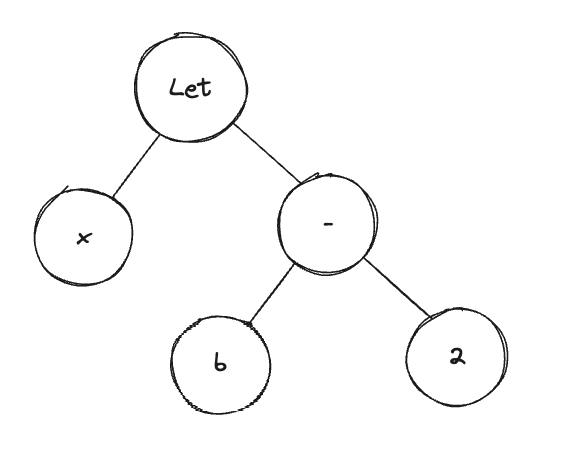
\includegraphics[width=6cm]{Screenshot 2024-04-22 at 18.59.30.png}
}

\bigskip

From this, the code generator would traverse the graph using pre-order traversal, recursively calling the \texttt{compile} method on each node, for instance, the compile method would be called on the parent root node, which would recursively call the same method on each of its child nodes. During compilation of the RHS node, it would also recursively compile its child nodes - until an assembly representation of the program is built up. The compile method generates a list of assembly language instructions which perform the behaviour specified for that particular operation. The assembly generated for this program would look as follows:
\begin{lstlisting}
// x variable is mapped to memory address $01 
ldi a, 2
sub b, a 
sw  $01, b
\end{lstlisting}
Depending on the number of working variables in memory, the register x may be assigned to one of the general purpose registers instead.

The unique method in which selection statements are compiled down into assembly code in the Jack compiler is useful to analyse due to the convenience it offers when writing a compiler - namely it allows you to ignore calculating offsets by taking full advantage of the higher level features of the assembler (a luxury afforded due to the two step compilation process). To compile selection statements in the Jack Compiler, the compiler generates a series of arbitrary labels e.g. (L1, L2) and places these after key points in the selective process in order to avoid offset calculating - a functionality that can be handled by the assembler. To compile the following:
\begin{lstlisting}
if (b > 10) {
    c = b;
} elif (b % 2 == 0) {
    b = b + 1; 
} else {
    b = b - 1;
}
\end{lstlisting}

The compiler will insert labels before the first instruction of each branch, and insert any code for the unconditional 'else' block after the jump instructions for any conditions (elif, and then branches). This approach avoids calculating any offsets and thus only a single pass is required to compile this program.

\begin{lstlisting}
// if b > 10 goto .then
ldi a, 10
sub a, b, a 
bgt .then

// elif b % 2 == 0 goto .elif
ldi a, 2
mod b, 2
beq .elif

// b = b - 1
lda a, 1
sub b, a
goto end

.then
    // c = b
    mov c, b
    goto end
.elif
    // b = b + 1
    ldi a, 1
    add b, a
.end
\end{lstlisting}

\subsubsubsection{Advantages \& Disadvantages}
The advantages of the Jack programming language include its specific keywords that offer insight into the manner in which its features are implemented - removing some of the abstraction typical higher level langauges offer. Another advantage is its type system, resulting in robust programs and reducing the edge cases a compiler would have to deal with. If an incorrect type was passed to a function or operation, an error would be thrown at compile time and no such error could occur in the compiled machine code.

However, the disadvantages of the Jack language include its Object Oriented approach making compilation difficult. Attribute variables on different instances of classes will have different  lifetimes and therefore freeing the finite number of registers the computer offers to make space for newly declared variables becomes much harder a task. Secondly, Jack uses many unecessary keywords, for instance the \texttt{do} keyword functioning as an abstraction for calling a method and ignoring its return value, and the \texttt{let} keyword being required every time you assign a variable rather than for its declaration alone. This means declarations in Jack are required to be sepereate statements, increasing the volume of code required to perform the same task.

\subsubsubsection{Takeaways}
The takeaways from this language include:
\begin{enumerate}
    \item Use a procedural aproach to program structure rather than an object oriented one.
    \item Limit the number of keywords used in the final source code to only those that offer useful insight into the purpose of statements in the program.
    \item Consider implementing a 2 step compilation process to take advantage of the assemblers higher level conveniences around labels and offsets.
    \item Use a simplified statically typed type system closer to that of Java or Go rather than Rust or C.
    \item Compile selection and iterative statements using generated labels rather than calculated offsets.
\end{enumerate}

\subsubsection{Austin Morlan's CHIP-8 Emulator}
CHIP-8 is a specification for a fictitious computer designed to provide an easy entry point into developing emulators, intended as a stepping stone before approaching more complex systems. I will analyse Austin Morlan's CHIP-8 emulator, \textcite{CHIP-8}, and discuss the manner in which he has realised the internal state of the computer through code and how this can be applied to my system.

First I will discuss the actual hardware of the CHIP-8 computer itself, in order to provide a background when discussing its implementation in code. The CHIP-8 system is an 8-bit general purpose, Von Neuman computer. It has 16 general purpose registers labelled \texttt{V0-VF} which can hold values ranging from \texttt{0x00-0xFF}, \textcite{CHIP-8-blog}. The \texttt{VF} flag is called the flag register, and its bits are set or unset depending on the result of calculations. For example, were the result of a calculation to be negative, the corresponding negative bit in the \texttt{VF} flag would be set.

CHIP-8 contains 4096 bytes of memory (from \texttt{0x000} to \texttt{0xFFF}) subdivided as follows: \texttt{0x000-0x1FF} contains the bootloader (a program to initialise the computer's state and begin execution of general purpose programs), \texttt{0x040-0x0A0} contains the computers character set (binary data containing the pixel representations of ASCII characters), and the rest of the memory is used to store instructions and data respectively.

CHIP-8 also contains a number of special purpose internal registers including a 16 bit Index register (I) used to store memory addresses for use in operations, and a 16 bit Program Counter (PC) that holds the address of the next instruction to execute, \textcite{CHIP-8-blog}. There is also an 8-bit Delay timer that decrements its value when non-zero - used to regularise time intervals between frames when writing games, and an 8-Bit Sound Timer that emits a buzz when its value is non-zero.

The CHIP-8 computer contains a 16-bit address stack of depth 16 referred to by an 8-bit stack pointer (SP) which keeps track of the most recent value pushed onto the stack. Whenever a \texttt{call} instruction is executed, the current value of the PC is pushed onto the top of the stack and SP incremented to point to this new value. Correpondingly, when a \texttt{ret} instruction is executed, the top value is popped off of the stack and set as the new value for the PC, causing program execution to resume after the \texttt{call} instruction.

Finally, CHIP-8 has memory-mapped I/O (where the input or output of peripherals are stored in main memory). For instance, 16 bits are used to represent the 16 keys of the CHIP-8 system with a 0 or 1 rerpesenting whether a key is held down. 2KB are used to store the 32*64 black and white monochrome display - with one bit per pixel.

Austin represented this internal state through the following class definition:
\begin{lstlisting}
#define CHARSET_ADDRESS  0x50
#define START_ADDRESS    0x200
#define MEMORY_SIZE      4096;
#define VIDEO_HEIGHT     32;
#define VIDEO_WIDTH      64;

class Chip8 {
    public:
        uint8_t registers[16];
        uint8_t memory[4096];
        uint16_t index;
        uint16_t pc;
        uint16_t stack[16];
        uint8_t sp;
        uint8_t delayTimer;
        uint8_t soundTimer;
        uint16_t opcode;
};
\end{lstlisting}

The scaffolding of Morlan's emulator revolves around an indefinite loop simulating the CPU's clock cycles, each of which contains the code to fetch, decode and execute instructions, \textcite{Muller-CHIP-8}. First the program fetches the 16-bit instruction from the address specified by the PC (and its following byte) and a bitmask is applied to extract the 4-bit opcode. A switch statement is then used to determine the operation and modify the internal state of the computer to carry out its behaviour accordingly by modifying register values or reading/writing to memory. Finally the timers are decremented should they be non-zero. 

\begin{lstlisting}
void chip8::emulateCycle() {
  // Fetch 16-bit instruction (4-bit opcode, 12-bit operand)
  instruction = memory[pc] << 8 | memory[pc + 1];
 
  // Decode opcode
  switch(instruction & 0xF000) {    
    case 0xA000: // ANNN: Sets I to the address NNN
      I = opcode & 0x0FFF;
      pc += 2;
    break;

    [...]
 
    default:
      printf ("Unknown opcode: 0x%X\n", opcode);
  }  
 
  // Update timers
  if(delay_timer > 0)
    --delay_timer;
 
  if(sound_timer > 0) {
    --sound_timer;
  }  
}
\end{lstlisting}

\subsubsubsection{User Interface}
Morlan has designed the UI for his emulator with 2 distinct parts, the display on the left, and the debugger on the right. The display is a graphical representation of the contents of VRAM, consisting in this case of a 32x64 pixel monochrome display. The debugger contains a dissassembled version of the currently executing instruction represented as a mneumonic, the contents of all special purpose registers (I, PC, SP), all general purpose registers (V0-VF), and the stack. This information allows a programmer to determine whether their code is running and registers being modified as expected, debugging their programs accordingly.

\bigskip

\shadowbox{
    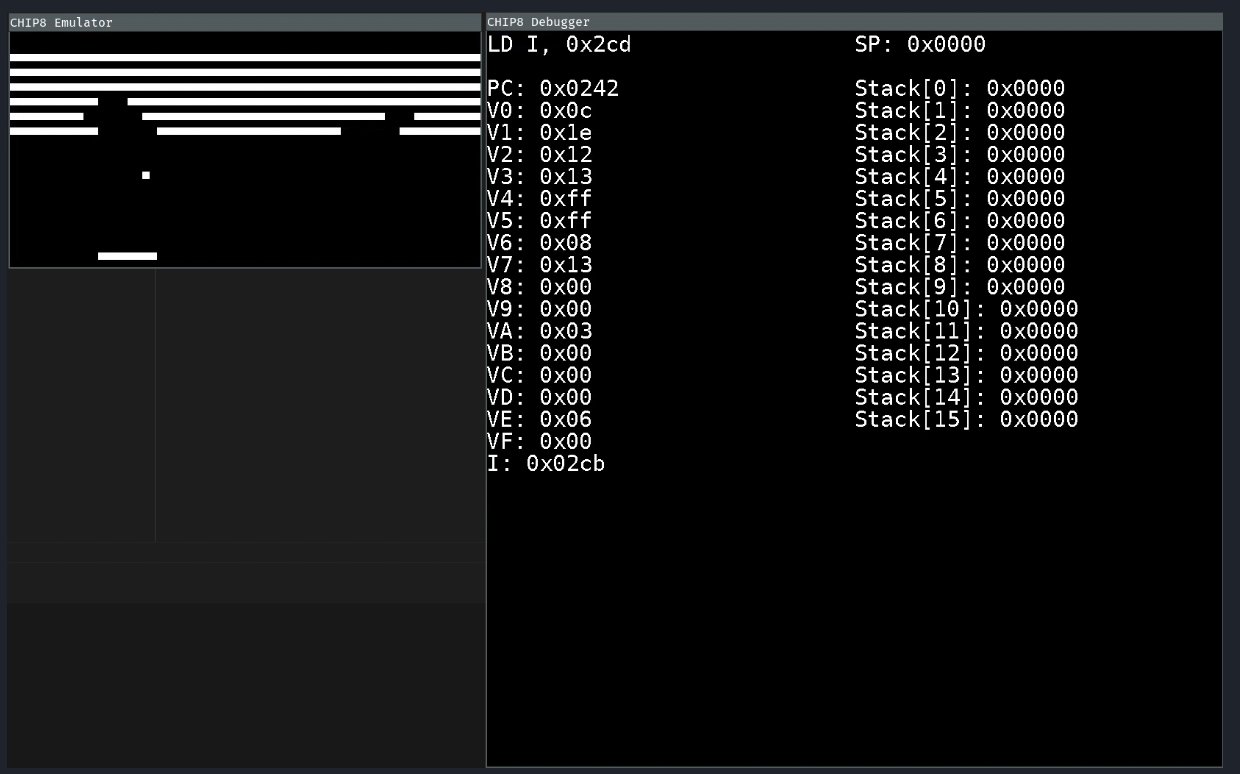
\includegraphics[width=12cm]{Screenshot 2024-04-27 at 16.02.09.png}
}

\subsubsubsection{Advantages \& Disadvantages}
Morlan has decided to increment the PC value inside the switch statement seperately for each instruction (\texttt{emulateCycle()} line 9), reducing a potential source of bugs. If the PC is incremented automatically at the end of the \texttt{emulateCycle()} method, should the PC be modified during the execution of an instruction (e.g. branch, call or return) then automatically incrementing the PC would offset its value from that which is intended. 

Morlan's debugger contains enough information to be of use to a programmer, however without a means to probe memory, lacks some of the functionality required. Furthermore, its prominent position in the UI overshadows the actual display, so a toggleable debugger would leave more room for the display itself.

Around the CHIP-8 system more generally, having memory addressable through 3 bytes (0x000-0xFFF or 4096 distinct memory locations) frees a nibble to represent the opcode, meaning an instruction can fit in a 16 bit register - since this is the same as the word size for the CHIP-8 processor, it means the system can fetch all instructions within a single cycle, increasing efficiency.

Furthermore, using a Delay timer rather than an interrupt-request system simplifies the process of synchronising CPU operations to real world timings, e.g. when drawing frameas for a simulation at a fixed frame rate, instead of polling (listening) for requests to trigger the code to draw a frame, only executing the code to draw the frame when the delay counter is 0 would have the same effect.

\subsubsubsection{Takeaways}
The takeaways from the CHIP-8 architecture and emulator include:
\begin{enumerate}
    \item Incrementing the PC should be done either inside the switch statement or after fetching the instruction to avoid modifying the PC multiple times and reduce a source of bugs.
    \item Design a togglable debugger that can be hidden when it is not required to prioritise space for the graphical display.
    \item Using a Delay timer rather than an interrupt-request system simplifies both the hardware and software side of the comptuer, avoiding the need to define Interrupt Request Tables (mapping interrupt codes to the Interrupt Service Request (ISR) required to service them).
\end{enumerate}

\subsection{Client Proposal}
My client is my uncle, a software engineer who has a keen curiosity around lower level development. He would like to learn how the everyday languages he uses to program are implemented on the most fundemental level. I will present him with the following proposal and assertain his thoughts on a series of questions to dictate the direction and design of my project.

My aim is to design a 16 bit processor with a RISC instruction set and the capability to execute complex programs such as tetris whilst interfacing with I/O devices such as a keyboard to handle input. I will build the suit of tools required to emulate the behaviour of such a processor. Firstly, a virtual machine, able to emulate the hardware of my processor and execute machine code programs with the correct clock timing and behaviour. This will include a simple GUI that reflects the contents of VRAM (Video RAM) allowing images and information to be communicated to the user.

Then, I will design the syntax of an assembly language that represents the machine code instructions of the processor's instruction set, and a multi-pass assembler to compile this down into binary machine code. The assembler should be able to calculate the required offsets of branch instructions from the position of labels in the source code, and potentially handle macro instruction expansions. (where pseudo-instructions represented by mneumonics can be defined - which at compile time are substituted for a list of fundemental instructions that carry out that defined task).

Finally, I will design a high level language with syntax similar to C and features such as iteration, procedures \& methods, selective statements, static typing, variables, references, and pointers. The experience of programming in this language should be familiar to anyone with programming experience, however remove some of the higher level abstractions typical languages offer, providing insight into the manner in which features are implemented. 

\subsubsection{Client Interview}
\label{sec:Interview}
I will interview my client to get his views on a number of questions regarding the design of my project, including the processor design and instruction set; the assembly language syntax and   machine code abstractions (macros and labels); and finally the higher level language syntax and features (OOP, first order functions, etc...).  
\begin{enumerate}
    \item \textbf{Instruction Set Architecture \& Assembler}
        \begin{itemize}
            \item Do you have any low level experience? \\
                \textit{"I used assembly when writing a driver a few years back, but I've not gone much lower level than that. Although I can remember some theory from University."}
            \item What architecture did you use, and what were your experiences using it? \\
                \textit{"I was migrating a driver in x86 to ARM so I've touched on both. x86 is definitely more powerful, but that does mean it has a steeper learning curve."}
            \item Did you prefer working with a CISC (x86) or RISC (arm) Instruction Set? \\
                \textit{"I tend to prefer RISC because the fewer instructions mean that those that are present tend to be much more carefully thought out, it's also just generally easier to program without flipping back to the documentation every 5 minutes."}
            \item Have you ever programmed for a Harvard architecture computer? \\
                \textit{"Most ARM processor tend to run on a Harvard architecture, although the assembly language hides most of that anyway so it's not something I really have to worry about."}
            \item What in particular did you like about the syntax of x86 or arm assembly?\\
                \textit{"They're both quite similar aside from their register names. x86 uses eax, ebx - but arm uses r0, r1.  Which I think makes more sense. I think x86 has longer menumonics as well - although that's probably because of its larger instruction set."}
            \item When writing assembly do you find yourself using labels or macro instructions?\\
                \textit{"Labels are vital, I use them everywhere. But for a RISC processor like arm - macro instructions provided by the assembler can be really helpful - they cut out a lot of the tedious programming when you write the same thing over and over."}
            \item Would you prefer to write assembly for a 16-bit or an 8-bit system? \\
                \textit{"I would prefer a 16-bit system because of the flexibility in representing large or precise numbers which you just can't do with an 8-bit system. It lets you worry less about overflow and underflow and all the quirks of binary maths."}
        \end{itemize}
        Takeaways:
        \begin{enumerate}
            \item My client favours a RISC instruction set, particularly the carefully considered instructions. I should take time when designing my instruction set to ensure there is enough breadth to cover all the desired functionality in an effective manner that is convenient to program in.
            \item My assembly language's instructions should abstract away the quirks of the Harvard architecture's seperate data and instruction memories - meaning my client will have more transferable experience when programming in my langauge.
            \item Registers should be named logically, either  alphabetically or numerically, e.g. 'r0, r1, r2, ...' or 'a, b, c, ...'.
            \item My client would prefer a 16-bit system.
        \end{enumerate}
    \item \textbf{Compiler \& High Level Language}
        \begin{itemize}
            \item When you write code, do you prefer an Object Oriented or Procedural Style? \\
                \textit{"I like the flexibility of the procedural approach, although I tend to write cleaner code when I use OOP. I just think it's too restrictive for smaller systems."}
            \item Do you prefer a simpler syntax like python, or something more like C? \\
                \textit{"I've been coding in Go recently for work and I like their approach. It's got the unambigious syntax of C with the flexibility in how you format your code, but they've also simplified the type system so you don't have to think about integer sizes or pointers in strings."}
            \item Would you like my language to have a simlar syntax to preexisting langauges, or to try something new? \\
                \textit{"I think it's important a language is readable to someone with no experience programming in it, so I wouldn't change the format too much. But it's nice to try some new things, like what go did with goroutines, or rust with the borrow checker."}
            \item If you could design your own language, what features would be most important to you? \\
                \textit{"I think good error messages go a long way into improving my experience with a language. They're often overlooked when you're writing a language, but for someone just learning how to code, they're make or break. I'd also say a good type system, Go and Java have pretty good approaches, although when you're writing something lower level you need that extra information about the size of your variables they just don't offer. What Rust does with it's numeric types is good, although I think their approach to strings needs refining."}
        \end{itemize}
        Takeaways:
        \begin{enumerate}
            \item My language should be a primarily procedural langauge, however offer optional elements of object oriented programming such as classes and interfaces to help organise programs.
            \item My programming language should use the C like syntax elements of curly braces and semi colons as they offer more flexibility when formatting code. 
            \item Without straying too far from the norms, I should consider alternative aproaches to syntax and langage features in order to differentiate my language, aggregating positive elements of other systems.
            \item My compiler should produce specific and actable error messages that are actually helpful to a programmer. This may include information on how to approach correcting such an error and its location in the source code. 
            \item A strong type system is important, It should abstract the implementation details of compound data structures such as strings, however still offer the flexibility required when writing lower level programs. For example specifying an integer size or whether it is signed or unsigned.
        \end{enumerate}
    \item \textbf{Virtual Machine}
        \begin{itemize}
            \item Have you ever used a Virtual Machine before? \\
                \textit{"I've used a Gameboy emulator before, but never anything for coding. I just haven't had the need."}
            \item What features would you expect if you were using developing using a virtual machine to test your code \\
                \textit{"I think a good debugger is important, certainly one showing the contents of RAM, register values, and the current instruction being executed. With maybe the ability to step through a program one instruction at a time setting breakpoints."}
        \end{itemize}
        Takeaways:
        \begin{enumerate}
            \item My virtual machine should include a comprehensive debugger for testing programs, you should be able to check the internal state of the computers memory and registers to determine whether the program is functioning as intended.
        \end{enumerate}
\end{enumerate}

This interview has affirmed that the direction in which to take my project is that of a simpler RISC processor with carefully considered instructions, relying more on macro instructions provided by the assembler to improve the development experience rather than on the hardware itself. My client also suggested a procedural language structure with syntax similar to C, a common trend with lower level languages. He also emphasised the importance of a well considered type system and error messages, so these should have careful consideration in my design section. Finally, due to the difficulty of testing machine code programs, a debugging mode in the virtual machine would greatly improve the experience of my client when writing assembly code.

\newpage
\subsection{Objectives}
\begin{longtable}{ | p{2cm} | p{4cm} | p{5cm} | p{4cm} | } 
    \hline
        Objective & Requirement & Justification & Deliverables \\ 
    \hline
        1.0 ISA \& Assembler & & & \\ 
    \hline
        1.1
        & 
        A RISC (Reduced Instruction Set Computer) design philosophy. 
        &
        A RISC instruction set can have better performance due to the faster and more efficient execution of it's instructions, especially when a user isn't as familiar with the instruction set of the system. (Client Interview 1.1) 
        & 
        \\
  \hline
        1.2 
        & 
        A Von Neuman computer architecture where data and instructions are stored in the same memory. 
        & 
        The shared memory between data and instructions minimises memory wastage since they can both share the same memory locations. (University of Washington MIPS Computer 1.) 
        & 
        \\
  \hline
        1.3 
        &  
        My Instruction Set should utilize 3 address operands standards.
        & 
        3 address operands is the programming standard for both arm and x86, pre-established instruction sets programemrs are already familiar with. The need to address instruction and data from different memories in a Harvard architecture is typically hidden from the programmer. (Client Interview 1.2)
        & 
        Assembly instructions should take 3 operands: a destination register followed by 1-2 source registers. Programmers should interface with the branch and load instructions in the same manner when addressing instructions or data.
        \\
  \hline
        1.4 
        & 
        Branch and call instructions should calculate offsets from labels in the source code. 
        & 
        Labels allow programmers to write branching or selective statements without having to manually calculate memory offests. (The Hack Computer, The University of Washington MIPS Computer, Client Interview) 
        & 
        My assembler should replace all occurences of a label in the assembly source code with calculated offests from the current instruction to that label.
        \\
  \hline
        1.5 
        & 
        Macro instructions to perform common tasks that are not otherwise specified in the ISA. 
        &
        Macro instructions minimise the need for programmers to repeat chunks of code to perform common tasks such as pushing values to the stack or calling functions. (The Hack Computer 2., Client Interview) 
        & 
        The assembler should substitute compound instructions such as \texttt{call} and \texttt{ret} for a list of machine code instructions that perform the same task.
        \\
    \hline
        1.6 
        & 
        A set of registers broad enough to minimse memory access. 
        &
        Prioritising registers over RAM improves processor performance as calculations can be performed with reduced latency. A delay timer simplifies the process of timing CPU operations, and a memory-resident address stack simplifies the process of calling and returning from functions. (Austin Moorlan's CHIP-8 Emulator, Client Interview 1.3)
        & 
        My processor should have 16 general purpose registers (r0-rF), a stack pointer (SP), program counter (PC), and delay timer (DT).
        \\
    \hline
        1.7 & 
        A CPU word length of 16-bits. &
        A 16-bit word length allow more bits to be processed in a single cycle and allows 16-bit instructions to be fetched within a single cycle improving performance. 16-bits can also represent numbers of a greater magnitude than 8-bits reducing overflow errors. (Client Interview 1.4) &
        Registers, ALU operations, memory locations and busses should all operate on 16-bit values.\\
    \hline
        2.0 Compiler & 
        &
        & 
       \\
    \hline
        2.1 & 
        C standard syntax with semi colons and braces rather than indentation. &
        This makes for easier compilation and more flexibility when formatting code, as well as reporting errors such as an unterminated brace at compile time (unlike incorrect indentation which may not be detected until debugging) (Client Interview 2.2) & 
        Lines should be terminated using a semi-colon, and curly-braces used to signify code blocks in selective or iterative expressions rather than indentation.\\
    \hline
        2.2 & 
        The programming language should be statically typed. &
        A type system ensures type-errors are thrown at compile time rather than during execution, leading to more robust programs that are easier to debug. Furthermore compilation becomes easier with statically typed variables as their size in memory is predetermined. (Monkey.2, Jack.4, Client Interview 2.5) & 
        My syntax should support signed and unsigned integers, strings, and integers of different sizes. The \texttt{let} keyword should be used when declaring a variable and require the type to be specified alongside its identifier. \\
    \hline
        2.3 & 
        The language should support a procedural programming paradigm. &
        Procedural programming is much more straightforward to compile since variable lifetimes within multiple instances and references of an object don't have to be calculated - simplifying the process of garbage collection. (Client Interview 2.1, Jack.1) & 
        All statements should be contained within methods, with the single entry point being a compulsory \texttt{main()} method. \\
    \hline
        2.4 & 
        My language should support references and pointers to variables in memory. & 
        Pointers allow programmers to implement arrays and strings by accessing variables through their memory location rather than an identifier. They also let you pass structs (otherwise a large data structure inefficient to pass as a copy) to a function as well as references to the first instruction of a function (allowing for first order functions) (Monkey.3)& 
        Programmers should be able to create a pointer to a variable: (\texttt{\&a}), and dereference it (\texttt{*a}). \\
    \hline
        2.5 & 
        The compiler should produce relevant error messages, pointing out the position in source code if relevant. &
        Relevant error messages make debugging much easier and improve the programmer's experience with a language. (Client Interview 2.4) &
        Error messages should include an easy to understand description of the error, its position in source code - and if possible, relevant steps to correcting it.
        \\
    \hline
        3.0 Virtual Machine & 
        &
        & 
       \\
    \hline
        3.1 & 
        The Virtual Machine should include a graphical display showing the contents of VRAM. &
        It makes programs more interactive and easily debuggable, as well as allowing programs such as simulations or games to be written for the system, expanding its capabilties. (Austin Morlan's CHIP-8 Emulator) & 
        \\
    \hline
        3.2 & 
        The Virtual Machine should include a togglable debugger. &
        A debugger would help programmers locate errors and test their programs, as well as ensuring the internal state of the computer is being modified as intended. (Client Interview 3.1, Austin Morlan's CHIP-8 Emulator.2) & 
        The debugger should show the contents of the general and special purpose registers, the currently executing instruction, and be able to probe the contents of memory. \\
        \hline
\end{longtable}
\newpage